%==============================================================================
% EECS 127 - Discussion 7: Convexity of Functions and Sets
%==============================================================================

\documentclass[10pt]{article}
\usepackage[margin=0.75in]{geometry}

%------------------------------------------------------------------------------
% REQUIRED PACKAGES
%------------------------------------------------------------------------------
\usepackage{amsmath, amssymb, amsthm}
\usepackage{microtype}
\usepackage{enumitem}
\usepackage{fancyhdr}
\usepackage{titlesec}
\usepackage{tcolorbox}
\usepackage{booktabs}
\usepackage{tikz}

%------------------------------------------------------------------------------
% SPACING
%------------------------------------------------------------------------------
\linespread{1.08}
\setlength{\parskip}{0.4ex plus 0.2ex minus 0.1ex}

%------------------------------------------------------------------------------
% BOX STYLES
%------------------------------------------------------------------------------
\tcbset{
    boxrule=0.8pt,
    colback=white,
    colframe=black,
    arc=0pt,
    boxsep=3pt,
    left=4pt, right=4pt, top=4pt, bottom=4pt
}

\newtcolorbox{result}{
    boxrule=0pt,
    colback=black!5,
    colframe=white,
    arc=0pt,
    boxsep=2pt,
    left=4pt, right=4pt, top=4pt, bottom=4pt
}

%------------------------------------------------------------------------------
% SECTION FORMATTING
%------------------------------------------------------------------------------
\titleformat{\section}{\large\bfseries}{\thesection.}{0.5em}{}
\titleformat{\subsection}{\normalsize\bfseries}{\thesubsection}{0.5em}{}
\titlespacing*{\section}{0pt}{1.5ex}{1ex}
\titlespacing*{\subsection}{0pt}{1ex}{0.5ex}

%------------------------------------------------------------------------------
% LIST FORMATTING
%------------------------------------------------------------------------------
\setlist{itemsep=1pt, topsep=3pt, parsep=1pt, leftmargin=1.5em}

%------------------------------------------------------------------------------
% HEADER/FOOTER
%------------------------------------------------------------------------------
\pagestyle{fancy}
\fancyhf{}
\fancyhead[L]{\small EECS 127}
\fancyhead[R]{\small Discussion 7}
\fancyfoot[C]{\small\thepage}
\renewcommand{\headrulewidth}{0.4pt}

%------------------------------------------------------------------------------
% THEOREM ENVIRONMENTS
%------------------------------------------------------------------------------
\theoremstyle{definition}
\newtheorem{definition}{Definition}
\newtheorem{example}{Example}

\theoremstyle{plain}
\newtheorem{theorem}{Theorem}
\newtheorem{lemma}{Lemma}

%------------------------------------------------------------------------------
% CUSTOM COMMANDS
%------------------------------------------------------------------------------
\newcommand{\RR}{\mathbb{R}}
\DeclareMathOperator{\dom}{dom}
\DeclareMathOperator{\epi}{epi}

%==============================================================================

\begin{document}

\noindent
\begin{minipage}{\linewidth}
    \centering
    \textbf{\Large Discussion 7: Convexity of Functions and Sets} \\[0.5em]
    \hrule
\end{minipage}
\vspace{1em}

%==============================================================================
\section{Background: What is Convexity?}
%==============================================================================

Convexity is one of the most important ideas in optimization. If a problem is ``convex,'' it becomes much easier to solve. This section builds everything from scratch.

\subsection{Convex Sets (the simpler idea; start here)}

\begin{definition}[Convex Set]
A set $C \subseteq \RR^n$ is \textbf{convex} if for every two points in the set, the entire straight line between them also stays inside the set.

Formally: for all $\vec{x}_1, \vec{x}_2 \in C$ and all $\theta \in [0,1]$:
\[
    \theta \vec{x}_1 + (1 - \theta)\vec{x}_2 \in C
\]
\end{definition}

\textbf{Let's unpack the formula.} The expression $\theta \vec{x}_1 + (1-\theta)\vec{x}_2$ is called a \textbf{convex combination}. As $\theta$ goes from 0 to 1, this expression traces out the line segment from $\vec{x}_2$ to $\vec{x}_1$:
\begin{itemize}
    \item When $\theta = 0$: the expression gives $0 \cdot \vec{x}_1 + 1 \cdot \vec{x}_2 = \vec{x}_2$ (the starting point).
    \item When $\theta = \frac{1}{2}$: the expression gives $\frac{1}{2}\vec{x}_1 + \frac{1}{2}\vec{x}_2$ (the midpoint).
    \item When $\theta = 1$: the expression gives $1 \cdot \vec{x}_1 + 0 \cdot \vec{x}_2 = \vec{x}_1$ (the ending point).
\end{itemize}

So the definition says: pick any two points in $C$, and every point on the line between them must also be in $C$.

\begin{example}[Concrete numbers]
Let $\vec{x}_1 = (2, 4)$ and $\vec{x}_2 = (6, 0)$. The point at $\theta = 0.3$ is:
\[
    0.3 \cdot (2,4) + 0.7 \cdot (6,0) = (0.6 + 4.2, \; 1.2 + 0) = (4.8, \; 1.2)
\]
For the set to be convex, $(4.8, 1.2)$ must be in the set.
\end{example}

\begin{example}[Convex vs. not convex]
\mbox{}

\begin{center}
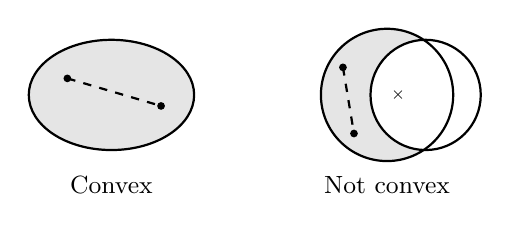
\begin{tikzpicture}[scale=0.7]
    % Convex: filled ellipse
    \fill[black!10] (0,0) ellipse (1.5 and 1);
    \draw[thick] (0,0) ellipse (1.5 and 1);
    \fill (-0.8,0.3) circle (2pt);
    \fill (0.9,-0.2) circle (2pt);
    \draw[thick, dashed] (-0.8,0.3) -- (0.9,-0.2);
    \node[below] at (0,-1.3) {\small Convex};

    % Not convex: crescent
    \begin{scope}[xshift=5cm]
        \fill[black!10] (0,0) circle (1.2);
        \fill[white] (0.7,0) circle (1);
        \draw[thick] (0,0) circle (1.2);
        \draw[thick] (0.7,0) circle (1);
        \fill (-0.8,0.5) circle (2pt);
        \fill (-0.6,-0.7) circle (2pt);
        \draw[thick, dashed] (-0.8,0.5) -- (-0.6,-0.7);
        \node at (0.2,0) {\tiny $\times$};
        \node[below] at (0,-1.3) {\small Not convex};
    \end{scope}
\end{tikzpicture}
\end{center}

\begin{itemize}
    \item \textbf{Left (convex):} An ellipse. Any line between two interior points stays inside.
    \item \textbf{Right (not convex):} A crescent. The dashed line passes through the ``bite'' taken out of the shape, leaving the set.
\end{itemize}
\end{example}

\begin{result}
\textbf{Common convex sets:}
\begin{itemize}
    \item A filled circle or ball: convex.
    \item A rectangle or box: convex.
    \item A halfspace $\{\vec{x} : \vec{a}^\top \vec{x} \le b\}$: convex. (Everything on one side of a flat boundary.)
    \item A single point: convex. A line: convex. All of $\RR^n$: convex. The empty set: convex.
\end{itemize}
\textbf{Common non-convex sets:}
\begin{itemize}
    \item A donut (annulus): not convex.
    \item The outside of a circle $\{(x,y) : x^2 + y^2 \ge 1\}$: not convex.
\end{itemize}
\end{result}

\subsection{Convex Functions}

\begin{definition}[Convex Function]
A function $f : \RR^n \to \RR$ is \textbf{convex} if two conditions hold:
\begin{enumerate}
    \item Its domain $\dom(f)$ is a convex set, and
    \item For all $\vec{x}, \vec{y} \in \dom(f)$ and $\theta \in [0,1]$:
    \[
        f\big(\theta \vec{x} + (1-\theta)\vec{y}\big) \le \theta f(\vec{x}) + (1-\theta)f(\vec{y})
    \]
\end{enumerate}
\end{definition}

\textbf{Let's understand each side of this inequality.}

\begin{itemize}
    \item \textbf{Left side:} $f\big(\theta \vec{x} + (1-\theta)\vec{y}\big)$. This is: ``first blend the inputs, then evaluate $f$.'' We take a point on the line between $\vec{x}$ and $\vec{y}$, and ask what is $f$ there?

    \item \textbf{Right side:} $\theta f(\vec{x}) + (1-\theta) f(\vec{y})$. This is: ``first evaluate $f$ at each endpoint, then blend the outputs.'' We compute $f$ at $\vec{x}$ and at $\vec{y}$, then take the same weighted average of those values.
\end{itemize}

The inequality says: the function value at the blended input $\le$ the blend of the function values. In other words, the function lies \emph{below} (or on) the line segment connecting the two points on its graph.

\begin{example}[Verifying $f(x) = x^2$ is convex with actual numbers]
Let $x = 1$, $y = 3$, $\theta = 0.5$ (midpoint). Check:
\begin{align*}
    \textbf{Left side: } &f(0.5 \cdot 1 + 0.5 \cdot 3) = f(2) = 4 \\
    \textbf{Right side: } &0.5 \cdot f(1) + 0.5 \cdot f(3) = 0.5 \cdot 1 + 0.5 \cdot 9 = 5
\end{align*}
Indeed $4 \le 5$. \checkmark \; The function at the midpoint ($= 4$) is below the average of the endpoint values ($= 5$).
\end{example}

\begin{tcolorbox}[colframe=black!50, title={\small Visual picture}]
\begin{center}
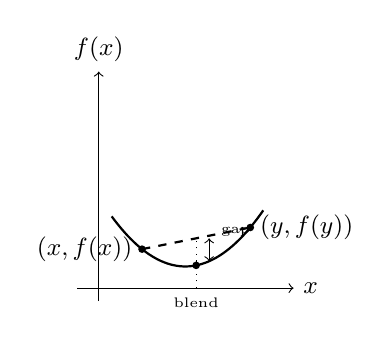
\begin{tikzpicture}[scale=0.55]
    \draw[->] (-0.5,0) -- (4.5,0) node[right] {\small $x$};
    \draw[->] (0,-0.3) -- (0,5) node[above] {\small $f(x)$};
    % Parabola
    \draw[thick, domain=0.3:3.8, samples=50] plot (\x, {0.4*(\x-2)*(\x-2)+0.5});
    % Chord
    \draw[thick, dashed] (1, {0.4*1+0.5}) -- (3.5, {0.4*2.25+0.5});
    % Points
    \fill (1, {0.4*1+0.5}) circle (2.5pt) node[left] {\small $(x, f(x))$};
    \fill (3.5, {0.4*2.25+0.5}) circle (2.5pt) node[right] {\small $(y, f(y))$};
    % Midpoint on curve
    \fill (2.25, {0.4*0.0625+0.5}) circle (2.5pt);
    % Midpoint on chord
    \draw[dotted] (2.25,0) -- (2.25, {0.5*(0.4*1+0.5) + 0.5*(0.4*2.25+0.5)});
    \node[below] at (2.25,0) {\tiny blend};
    % Arrow showing gap
    \draw[<->] (2.55, {0.4*0.3025+0.5}) -- (2.55, {0.4*1*0.5+0.5 + 0.5*(0.4*2.25)});
    \node[right] at (2.6, 1.3) {\tiny gap};
\end{tikzpicture}
\end{center}

The solid curve is $f$. The dashed line connects two points on $f$. Convexity means the curve always stays below (or on) the dashed line. The ``gap'' is the difference: right side minus left side $\ge 0$.
\end{tcolorbox}

\begin{result}
\textbf{Familiar convex functions:}
\begin{itemize}
    \item $f(x) = x^2$: parabola curving up.
    \item $f(x) = |x|$: V-shape.
    \item $f(x) = e^x$: exponential.
    \item $f(\vec{x}) = \vec{a}^\top \vec{x} + b$: any linear/affine function is both convex and concave.
\end{itemize}
\textbf{Familiar concave functions} (curve downward):
\begin{itemize}
    \item $f(x) = \log(x)$ for $x > 0$.
    \item $f(x) = \sqrt{x}$ for $x \ge 0$.
    \item $f(x) = -x^2$: upside-down parabola.
\end{itemize}
\end{result}

\subsection{Concave Functions}

\begin{definition}[Concave Function]
$f$ is \textbf{concave} if $-f$ is convex. Equivalently, the inequality flips:
\[
    f(\theta \vec{x} + (1-\theta)\vec{y}) \ge \theta f(\vec{x}) + (1-\theta)f(\vec{y})
\]
\end{definition}

The function lies \emph{above} the line segment. A function that curves downward (like $\log$ or $\sqrt{x}$) is concave.

\textbf{Special case:} Any affine function $f(\vec{x}) = \vec{a}^\top \vec{x} + b$ satisfies both $\le$ and $\ge$ with equality, so it is both convex and concave.

\subsection{The Epigraph}

\begin{definition}[Epigraph]
The \textbf{epigraph} of $f$ is the set of all points ``on or above'' the graph:
\[
    \epi(f) = \{(\vec{x}, t) : \vec{x} \in \dom(f), \; t \ge f(\vec{x})\}
\]
\end{definition}

Think of it this way: plot $f$ in $n+1$ dimensions (the input plus one extra axis for the output). Now shade everything above the surface. That shaded region is the epigraph.

\begin{example}[Epigraph of $f(x) = x^2$]
\mbox{}

\begin{center}
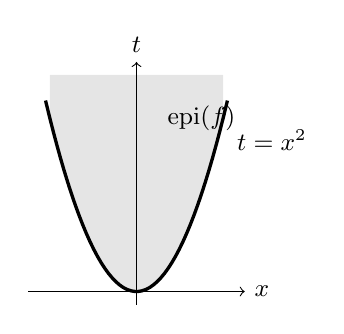
\begin{tikzpicture}[scale=0.55]
    \fill[black!10, domain=-2:2, samples=50] plot (\x, {\x*\x}) -- (2,5) -- (-2,5) -- cycle;
    \draw[->] (-2.5,0) -- (2.5,0) node[right] {\small $x$};
    \draw[->] (0,-0.3) -- (0,5.3) node[above] {\small $t$};
    \draw[very thick, domain=-2.1:2.1, samples=50] plot (\x, {\x*\x});
    \node at (1.5, 4) {\small $\epi(f)$};
    \node[right] at (2.1, 3.5) {\small $t = x^2$};
\end{tikzpicture}
\end{center}

The shaded region (above the parabola) is the epigraph. It is a convex set, which reflects the fact that $x^2$ is a convex function.
\end{example}

\begin{result}
\textbf{Key connection:} $f$ is convex $\iff$ $\epi(f)$ is a convex set.

This is powerful because it lets us translate between function convexity and set convexity.
\end{result}

\subsection{Three Tests for Convexity}

\begin{result}
\textbf{Test 1: Definition (works for any function, even non-differentiable).}
Check the inequality directly:
\[
    f(\theta \vec{x} + (1-\theta)\vec{y}) \le \theta f(\vec{x}) + (1-\theta)f(\vec{y})
\]
\end{result}

\begin{result}
\textbf{Test 2: First-order condition (requires $f$ differentiable).}
$f$ is convex $\iff$ for all $\vec{x}, \vec{y}$:
\[
    f(\vec{y}) \ge f(\vec{x}) + \nabla f(\vec{x})^\top (\vec{y} - \vec{x})
\]
\textbf{What $\nabla f(\vec{x})$ is:} The gradient of $f$ at $\vec{x}$, a vector of partial derivatives. The right side is the tangent line (or tangent plane) at $\vec{x}$. The condition says: a convex function always lies above all its tangent lines.
\end{result}

\begin{result}
\textbf{Test 3: Second-order condition (requires $f$ twice differentiable).}
$f$ is convex $\iff$ the Hessian matrix $\nabla^2 f(\vec{x})$ is positive semidefinite (PSD) everywhere.

\textbf{What the Hessian is:} The $n \times n$ matrix of all second partial derivatives. Positive semidefinite means all eigenvalues $\ge 0$.

\textbf{For single-variable functions:} This simplifies to $f''(x) \ge 0$ for all $x$. (The second derivative is nonnegative everywhere.)
\end{result}

\begin{example}[Checking $f(x) = x^2$ with all three tests]
\mbox{}

\textbf{Test 1:} $(\theta a + (1-\theta)b)^2 \le \theta a^2 + (1-\theta)b^2$? Yes, this is equivalent to $\theta(1-\theta)(a-b)^2 \ge 0$, which is always true.

\textbf{Test 2:} $f'(x) = 2x$. Check: $y^2 \ge x^2 + 2x(y - x) = 2xy - x^2$. This simplifies to $(y-x)^2 \ge 0$. True. \checkmark

\textbf{Test 3:} $f''(x) = 2 > 0$. Positive everywhere. \checkmark
\end{example}

\subsection{Jensen's Inequality}

\begin{result}
\textbf{Jensen's Inequality:} If $f$ is convex and $\theta_1 + \theta_2 + \cdots + \theta_k = 1$ with all $\theta_i \ge 0$:
\[
    f(\theta_1 \vec{x}_1 + \cdots + \theta_k \vec{x}_k) \le \theta_1 f(\vec{x}_1) + \cdots + \theta_k f(\vec{x}_k)
\]
\end{result}

This is just the convexity definition extended from 2 points to $k$ points. It says: ``the function at the weighted average is at most the weighted average of the function values.''

%==============================================================================
\section{Problem 1(a): Restriction to a Line}
%==============================================================================

\textbf{Problem:} Show that $f$ is convex if and only if for all $\vec{x} \in \dom(f)$ and all $\vec{v}$, the function $g(t) = f(\vec{x} + t\vec{v})$ is convex.

\subsection{What is $g(t) = f(\vec{x} + t\vec{v})$?}

This is a way to turn a multivariate function into a single-variable function by ``slicing'' it along a line.

\begin{tcolorbox}[colframe=black!50, title={\small Building intuition step by step}]
Imagine $f$ is a function on $\RR^2$ (like a hilly landscape).

\textbf{Step 1:} Pick a starting point $\vec{x}$. This is a specific location on the landscape.

\textbf{Step 2:} Pick a direction $\vec{v}$. This is the direction you will walk.

\textbf{Step 3:} As you vary $t$, the point $\vec{x} + t\vec{v}$ moves along a straight line through $\vec{x}$ in direction $\vec{v}$. When $t = 0$, you are at $\vec{x}$. When $t > 0$, you move forward. When $t < 0$, you move backward.

\textbf{Step 4:} $g(t) = f(\vec{x} + t\vec{v})$ records the ``altitude'' as you walk. It is a 1D function of the single variable $t$.

\textbf{The claim:} $f$ (the whole landscape) is convex if and only if $g$ (the altitude profile along every possible line) is convex.
\end{tcolorbox}

\begin{example}[With actual numbers]
Let $f(x_1, x_2) = x_1^2 + x_2^2$. Pick $\vec{x} = (1, 0)$ and $\vec{v} = (1, 2)$.

Then $\vec{x} + t\vec{v} = (1 + t, \; 2t)$, so:
\[
    g(t) = f(1 + t, \; 2t) = (1+t)^2 + (2t)^2 = 1 + 2t + t^2 + 4t^2 = 5t^2 + 2t + 1
\]
This is a quadratic in $t$ with positive leading coefficient ($5 > 0$), so it is a convex function of $t$. \checkmark
\end{example}

\subsection{Proof: ($\Rightarrow$) $f$ convex implies $g$ convex}

\textbf{Goal:} Assume $f$ is convex. Show $g(t) = f(\vec{x} + t\vec{v})$ is convex.

\textbf{What we need to show:} For any $t_1, t_2$ and $\lambda \in [0,1]$:
\[
    g(\lambda t_1 + (1-\lambda) t_2) \le \lambda g(t_1) + (1-\lambda) g(t_2)
\]

\textbf{Step 1: Write out the left side using the definition of $g$.}
\[
    g(\lambda t_1 + (1-\lambda)t_2) = f\big(\vec{x} + (\lambda t_1 + (1-\lambda)t_2)\vec{v}\big)
\]

\textbf{Step 2: Rearrange the argument of $f$ into a convex combination.}

This is the key algebraic manipulation. Distribute $\vec{v}$:
\[
    \vec{x} + (\lambda t_1 + (1-\lambda)t_2)\vec{v} = \vec{x} + \lambda t_1 \vec{v} + (1-\lambda) t_2 \vec{v}
\]

Now we use a trick: since $\lambda + (1-\lambda) = 1$, we can write $\vec{x} = \lambda \vec{x} + (1-\lambda)\vec{x}$:
\begin{align*}
    &= \lambda \vec{x} + (1-\lambda)\vec{x} + \lambda t_1 \vec{v} + (1-\lambda) t_2 \vec{v} \\
    &= \lambda(\vec{x} + t_1 \vec{v}) + (1-\lambda)(\vec{x} + t_2 \vec{v})
\end{align*}

This is a convex combination of $(\vec{x} + t_1 \vec{v})$ and $(\vec{x} + t_2 \vec{v})$.

\textbf{Step 3: Apply convexity of $f$.}

Since $f$ is convex and we have a convex combination:
\begin{align*}
    f\big(\lambda(\vec{x} + t_1 \vec{v}) + (1-\lambda)(\vec{x} + t_2 \vec{v})\big) &\le \lambda f(\vec{x} + t_1 \vec{v}) + (1-\lambda) f(\vec{x} + t_2 \vec{v}) \\
    &= \lambda g(t_1) + (1-\lambda) g(t_2)
\end{align*}

\textbf{Step 4: Combine.}

Putting Steps 1--3 together:
\[
    g(\lambda t_1 + (1-\lambda) t_2) \le \lambda g(t_1) + (1-\lambda) g(t_2)
\]
This is exactly the definition of $g$ being convex. $\square$

\begin{tcolorbox}[colframe=black!50, title={\small Step 2 is the only hard part}]
The entire proof boils down to one algebraic trick: splitting $\vec{x}$ into $\lambda \vec{x} + (1-\lambda)\vec{x}$ and regrouping. Everything else is just applying definitions. If you remember this trick, you can reproduce the proof.
\end{tcolorbox}

\subsection{Proof: ($\Leftarrow$) Every $g$ convex implies $f$ convex}

\textbf{Goal:} Assume $g(t) = f(\vec{x} + t\vec{v})$ is convex for every choice of $\vec{x}$ and $\vec{v}$. Show $f$ is convex.

\textbf{What we need to show:} For any $\vec{x}_1, \vec{x}_2 \in \dom(f)$ and $\lambda \in [0,1]$:
\[
    f(\lambda \vec{x}_1 + (1-\lambda)\vec{x}_2) \le \lambda f(\vec{x}_1) + (1-\lambda) f(\vec{x}_2)
\]

\textbf{Step 1: Cleverly choose $\vec{x}$ and $\vec{v}$ to define $g$.}

Set $\vec{x} = \vec{x}_2$ and $\vec{v} = \vec{x}_1 - \vec{x}_2$. Then define:
\[
    g(t) = f(\vec{x}_2 + t(\vec{x}_1 - \vec{x}_2))
\]

\textbf{Step 2: Check what $g$ gives at specific values of $t$.}
\begin{itemize}
    \item $g(0) = f(\vec{x}_2 + 0 \cdot (\vec{x}_1 - \vec{x}_2)) = f(\vec{x}_2)$
    \item $g(1) = f(\vec{x}_2 + 1 \cdot (\vec{x}_1 - \vec{x}_2)) = f(\vec{x}_1)$
    \item $g(\lambda) = f(\vec{x}_2 + \lambda(\vec{x}_1 - \vec{x}_2)) = f(\lambda \vec{x}_1 + (1-\lambda)\vec{x}_2)$
\end{itemize}

Note: $\vec{x}_2 + \lambda(\vec{x}_1 - \vec{x}_2) = \vec{x}_2 + \lambda \vec{x}_1 - \lambda \vec{x}_2 = \lambda \vec{x}_1 + (1-\lambda)\vec{x}_2$. This is just algebra.

\textbf{Step 3: Apply convexity of $g$.}

$g$ is convex by assumption. Apply the definition with inputs $t_1 = 1$, $t_2 = 0$, and weight $\lambda$:
\[
    g(\lambda \cdot 1 + (1-\lambda) \cdot 0) \le \lambda \cdot g(1) + (1-\lambda) \cdot g(0)
\]

\textbf{Step 4: Substitute the values from Step 2.}

The left side is $g(\lambda) = f(\lambda \vec{x}_1 + (1-\lambda)\vec{x}_2)$.

The right side is $\lambda g(1) + (1-\lambda)g(0) = \lambda f(\vec{x}_1) + (1-\lambda)f(\vec{x}_2)$.

So:
\[
    f(\lambda \vec{x}_1 + (1-\lambda)\vec{x}_2) \le \lambda f(\vec{x}_1) + (1-\lambda)f(\vec{x}_2)
\]

This is exactly the definition of $f$ being convex. $\square$

\begin{tcolorbox}[colframe=black!50, title={\small Intuition: Why this result is useful}]
Checking if a function on $\RR^{100}$ is convex sounds hard. But this result says: just check if every 1D slice is convex. And for a 1D function, convexity is easy to check (just verify $g''(t) \ge 0$).
\end{tcolorbox}

%==============================================================================
\section{Problem 1(b): Pointwise Maximum}
%==============================================================================

\textbf{Problem:} If $f_1$ and $f_2$ are convex, show that $f(\vec{x}) = \max(f_1(\vec{x}), f_2(\vec{x}))$ is convex.

\subsection{What is the pointwise maximum?}

At each point $\vec{x}$, we evaluate both $f_1(\vec{x})$ and $f_2(\vec{x})$, and take whichever is larger.

\begin{example}[Concrete]
Let $f_1(x) = 2x + 1$ and $f_2(x) = -x + 4$ (both lines, hence convex).
\begin{center}
\begin{tabular}{@{}cccc@{}}
\toprule
$x$ & $f_1(x)$ & $f_2(x)$ & $f(x) = \max$ \\
\midrule
0 & 1 & 4 & 4 \\
1 & 3 & 3 & 3 \\
2 & 5 & 2 & 5 \\
\bottomrule
\end{tabular}
\end{center}
The graph of $f$ follows $f_2$ when $x < 1$ and $f_1$ when $x > 1$, creating a V-shape: still convex.
\end{example}

\subsection{Proof 1: Via Epigraphs (most elegant)}

\textbf{The idea:} We will show that $\epi(f) = \epi(f_1) \cap \epi(f_2)$, then use the fact that intersections of convex sets are convex.

\textbf{Step 1: Check the domain.}

$\dom(f) = \dom(f_1) \cap \dom(f_2)$. We will prove in Problem 2 that the intersection of convex sets is convex, so $\dom(f)$ is convex. \checkmark

\textbf{Step 2: Write out what $\epi(f)$ is.}

\begin{align*}
    \epi(f) &= \{(\vec{x}, t) : f(\vec{x}) \le t\} \\
            &= \{(\vec{x}, t) : \max(f_1(\vec{x}), f_2(\vec{x})) \le t\}
\end{align*}

\textbf{Step 3: Simplify $\max(a, b) \le t$.}

The inequality $\max(a, b) \le t$ is true if and only if \emph{both} $a \le t$ and $b \le t$. (The larger of the two is at most $t$, so both must be at most $t$.)

\begin{align*}
    \epi(f) &= \{(\vec{x}, t) : f_1(\vec{x}) \le t \text{ and } f_2(\vec{x}) \le t\} \\
            &= \{(\vec{x}, t) : f_1(\vec{x}) \le t\} \;\cap\; \{(\vec{x}, t) : f_2(\vec{x}) \le t\} \\
            &= \epi(f_1) \cap \epi(f_2)
\end{align*}

\textbf{Step 4: Conclude.}

$f_1, f_2$ convex $\Rightarrow$ $\epi(f_1), \epi(f_2)$ are convex sets $\Rightarrow$ $\epi(f_1) \cap \epi(f_2)$ is convex (intersection of convex sets) $\Rightarrow$ $\epi(f)$ is convex $\Rightarrow$ $f$ is convex. $\square$

\begin{tcolorbox}[colframe=black!50, title={\small Why this proof is nice}]
It turns a question about functions into a question about sets. The key fact $\max(a,b) \le t \iff a \le t \text{ and } b \le t$ converts the pointwise max into an intersection.
\end{tcolorbox}

\subsection{Proof 2: Direct from the definition (most concrete)}

\textbf{Step 1: Set up.}

Take $\vec{x}_1, \vec{x}_2 \in \dom(f)$, $\lambda \in [0,1]$. Let $\vec{z} = \lambda \vec{x}_1 + (1-\lambda)\vec{x}_2$. We need:
\[
    f(\vec{z}) \le \lambda f(\vec{x}_1) + (1-\lambda) f(\vec{x}_2)
\]

\textbf{Step 2: Case split on which function achieves the max at $\vec{z}$.}

Since $f(\vec{z}) = \max(f_1(\vec{z}), f_2(\vec{z}))$, either $f(\vec{z}) = f_1(\vec{z})$ or $f(\vec{z}) = f_2(\vec{z})$.

\textit{Case 1: $f(\vec{z}) = f_1(\vec{z})$.}
\begin{align*}
    f(\vec{z}) &= f_1(\lambda \vec{x}_1 + (1-\lambda)\vec{x}_2) \\
               &\le \lambda f_1(\vec{x}_1) + (1-\lambda) f_1(\vec{x}_2) & \text{(convexity of $f_1$)}\\
               &\le \lambda \underbrace{\max(f_1(\vec{x}_1), f_2(\vec{x}_1))}_{= f(\vec{x}_1)} + (1-\lambda) \underbrace{\max(f_1(\vec{x}_2), f_2(\vec{x}_2))}_{= f(\vec{x}_2)} & \text{(since $f_i \le \max$)}
\end{align*}

The second inequality uses: $f_1(\vec{x}_1) \le \max(f_1(\vec{x}_1), f_2(\vec{x}_1))$ (a number is at most the max of it and something else). Same for $f_1(\vec{x}_2)$.

\textit{Case 2: $f(\vec{z}) = f_2(\vec{z})$.} Identical, with $f_2$ in place of $f_1$.

In both cases, $f(\vec{z}) \le \lambda f(\vec{x}_1) + (1-\lambda)f(\vec{x}_2)$. $\square$

\subsection{Proof 3: Using a lemma about max}

\textbf{Step 1: Prove a useful inequality.}

\begin{result}
\textbf{Lemma:} For any real numbers $a, b, c, d$:
\[
    \max(a + b, \; c + d) \le \max(a, c) + \max(b, d)
\]
\textbf{Proof of lemma:} We know $a \le \max(a,c)$ and $b \le \max(b,d)$. Adding: $a + b \le \max(a,c) + \max(b,d)$. Similarly, $c + d \le \max(a,c) + \max(b,d)$. Since both $a + b$ and $c + d$ are $\le$ the right side, so is their max. $\square$
\end{result}

\textbf{Step 2: Chain the inequalities.}
\begin{align*}
    &f(\lambda \vec{x}_1 + (1-\lambda)\vec{x}_2) \\
    &= \max\big(f_1(\lambda \vec{x}_1 + (1-\lambda)\vec{x}_2), \; f_2(\lambda \vec{x}_1 + (1-\lambda)\vec{x}_2)\big) \\
    &\le \max\big(\lambda f_1(\vec{x}_1) + (1-\lambda) f_1(\vec{x}_2), \; \lambda f_2(\vec{x}_1) + (1-\lambda) f_2(\vec{x}_2)\big) \\
    &\le \max\big(\lambda f_1(\vec{x}_1), \lambda f_2(\vec{x}_1)\big) + \max\big((1-\lambda) f_1(\vec{x}_2), (1-\lambda) f_2(\vec{x}_2)\big) \\
    &= \lambda \max(f_1(\vec{x}_1), f_2(\vec{x}_1)) + (1-\lambda)\max(f_1(\vec{x}_2), f_2(\vec{x}_2)) \\
    &= \lambda f(\vec{x}_1) + (1-\lambda) f(\vec{x}_2) \quad \square
\end{align*}

\textbf{Explanation of each line:}
\begin{itemize}
    \item Line 1 $\to$ 2: Apply convexity of $f_1$ and $f_2$ inside the max. Each $f_i$ at the blend $\le$ blend of $f_i$ values.
    \item Line 2 $\to$ 3: Apply the lemma.
    \item Line 3 $\to$ 4: Factor out $\lambda$ and $(1-\lambda)$. For example, $\max(\lambda a, \lambda b) = \lambda \max(a, b)$ when $\lambda \ge 0$.
\end{itemize}

\begin{tcolorbox}[colframe=black!50, title={\small Generalization}]
This extends to any number of functions: if $f_1, \ldots, f_m$ are all convex, then $f(\vec{x}) = \max_i f_i(\vec{x})$ is convex. This even works for infinitely many functions: $f(\vec{x}) = \sup_{\alpha} f_\alpha(\vec{x})$ is convex if every $f_\alpha$ is convex.
\end{tcolorbox}

%==============================================================================
\section{Problem 2(a): Intersection of Convex Sets}
%==============================================================================

\textbf{Problem:} If $C_1$ and $C_2$ are convex sets, show $C = C_1 \cap C_2$ is convex.

\subsection{What is $C_1 \cap C_2$?}

$C_1 \cap C_2$ is the set of points that are in \emph{both} $C_1$ and $C_2$ simultaneously: the overlap region.

\begin{example}
If $C_1$ is a circle and $C_2$ is a rectangle (both convex), their intersection is a ``rounded rectangle'' shape, which is also convex.
\end{example}

\subsection{Proof}

\textbf{Step 1: Take two arbitrary points in $C$.}

Let $\vec{x}_1, \vec{x}_2 \in C = C_1 \cap C_2$ and $\theta \in [0,1]$.

Since $\vec{x}_1 \in C_1 \cap C_2$, we know:
\begin{itemize}
    \item $\vec{x}_1 \in C_1$ \quad and \quad $\vec{x}_1 \in C_2$
\end{itemize}
Similarly:
\begin{itemize}
    \item $\vec{x}_2 \in C_1$ \quad and \quad $\vec{x}_2 \in C_2$
\end{itemize}

\textbf{Step 2: Apply convexity of $C_1$.}

$C_1$ is convex, and $\vec{x}_1, \vec{x}_2 \in C_1$, so by definition of convex set:
\[
    \theta \vec{x}_1 + (1-\theta)\vec{x}_2 \in C_1 \quad \checkmark
\]

\textbf{Step 3: Apply convexity of $C_2$.}

$C_2$ is convex, and $\vec{x}_1, \vec{x}_2 \in C_2$, so:
\[
    \theta \vec{x}_1 + (1-\theta)\vec{x}_2 \in C_2 \quad \checkmark
\]

\textbf{Step 4: Conclude.}

The point $\theta \vec{x}_1 + (1-\theta)\vec{x}_2$ is in $C_1$ (by Step 2) and in $C_2$ (by Step 3). Therefore it is in $C_1 \cap C_2 = C$. $\square$

\begin{tcolorbox}[colframe=black!50, title={\small The logic in one sentence}]
Each set individually ``keeps'' the convex combination inside. Since both sets keep it, the intersection keeps it too.
\end{tcolorbox}

\begin{result}
\textbf{This generalizes:} The intersection of \emph{any} number of convex sets (even infinitely many) is convex. The proof is identical: if the point is in every set, convexity of each set keeps the convex combination in that set, so the combination is in the intersection.
\end{result}

\begin{tcolorbox}[colframe=black!50]
\textbf{Warning: Union does NOT preserve convexity.}

Consider $C_1 = \{(x,y) : x \le -1\}$ and $C_2 = \{(x,y) : x \ge 1\}$. Both are convex (halfspaces). But $C_1 \cup C_2$ is not convex: the point $(-1, 0) \in C_1$ and $(1, 0) \in C_2$, but the midpoint $(0, 0)$ is in neither.
\end{tcolorbox}

\begin{tcolorbox}[colframe=black!50, title={\small Why this result matters in practice}]
\textbf{Feasible sets in optimization are intersections of constraints.} Each constraint like $\vec{a}^\top \vec{x} \le b$ defines a halfspace (convex). A system of constraints defines their intersection, which is convex by this result. This is why linear programs and convex programs have nice feasible sets.
\end{tcolorbox}

%==============================================================================

\vfill

\begin{center}
\rule{0.5\linewidth}{0.4pt}

\textit{Key Takeaways}
\end{center}

\begin{enumerate}
    \item \textbf{Convex set:} Every line between two points stays inside. \textbf{Convex function:} The graph lies below every chord.

    \item \textbf{Restriction to a line:} $f$ is convex if and only if every 1D slice $g(t) = f(\vec{x} + t\vec{v})$ is convex. The proof trick is writing $\vec{x} = \lambda\vec{x} + (1-\lambda)\vec{x}$.

    \item \textbf{Pointwise max preserves convexity.} Three ways to prove it: epigraph intersection, case-splitting, or the max-of-sums lemma. The epigraph proof uses the key equivalence $\max(a,b) \le t \iff a \le t$ and $b \le t$.

    \item \textbf{Intersection preserves set convexity} (but union does not). Each constraint in an optimization problem is a convex set; their intersection (the feasible set) is also convex.
\end{enumerate}

\end{document}
